\section{Untersuchung der Kinematik}
Der erste Schritt in der Modellbildung besteht in der Definition der Bezugssysteme, die zur Beschreibung der Systembewegung dienen. Der Ausgangspunkt ist das Inertialsystem $A$, welches durch die drei Einheitsvektoren $\bs{a}\idx1$, $\bs{a}\idx2$ und $\bs{a}\idx3$ definiert wird. Das Würfelgehäuse verfügt über drei rotatorische Freiheitsgrade, welche durch die Winkel $\varphi\idx1$, $\varphi\idx2$ und $\varphi\idx3$ beschrieben werden. 
\begin{figure}[!h]
\centering
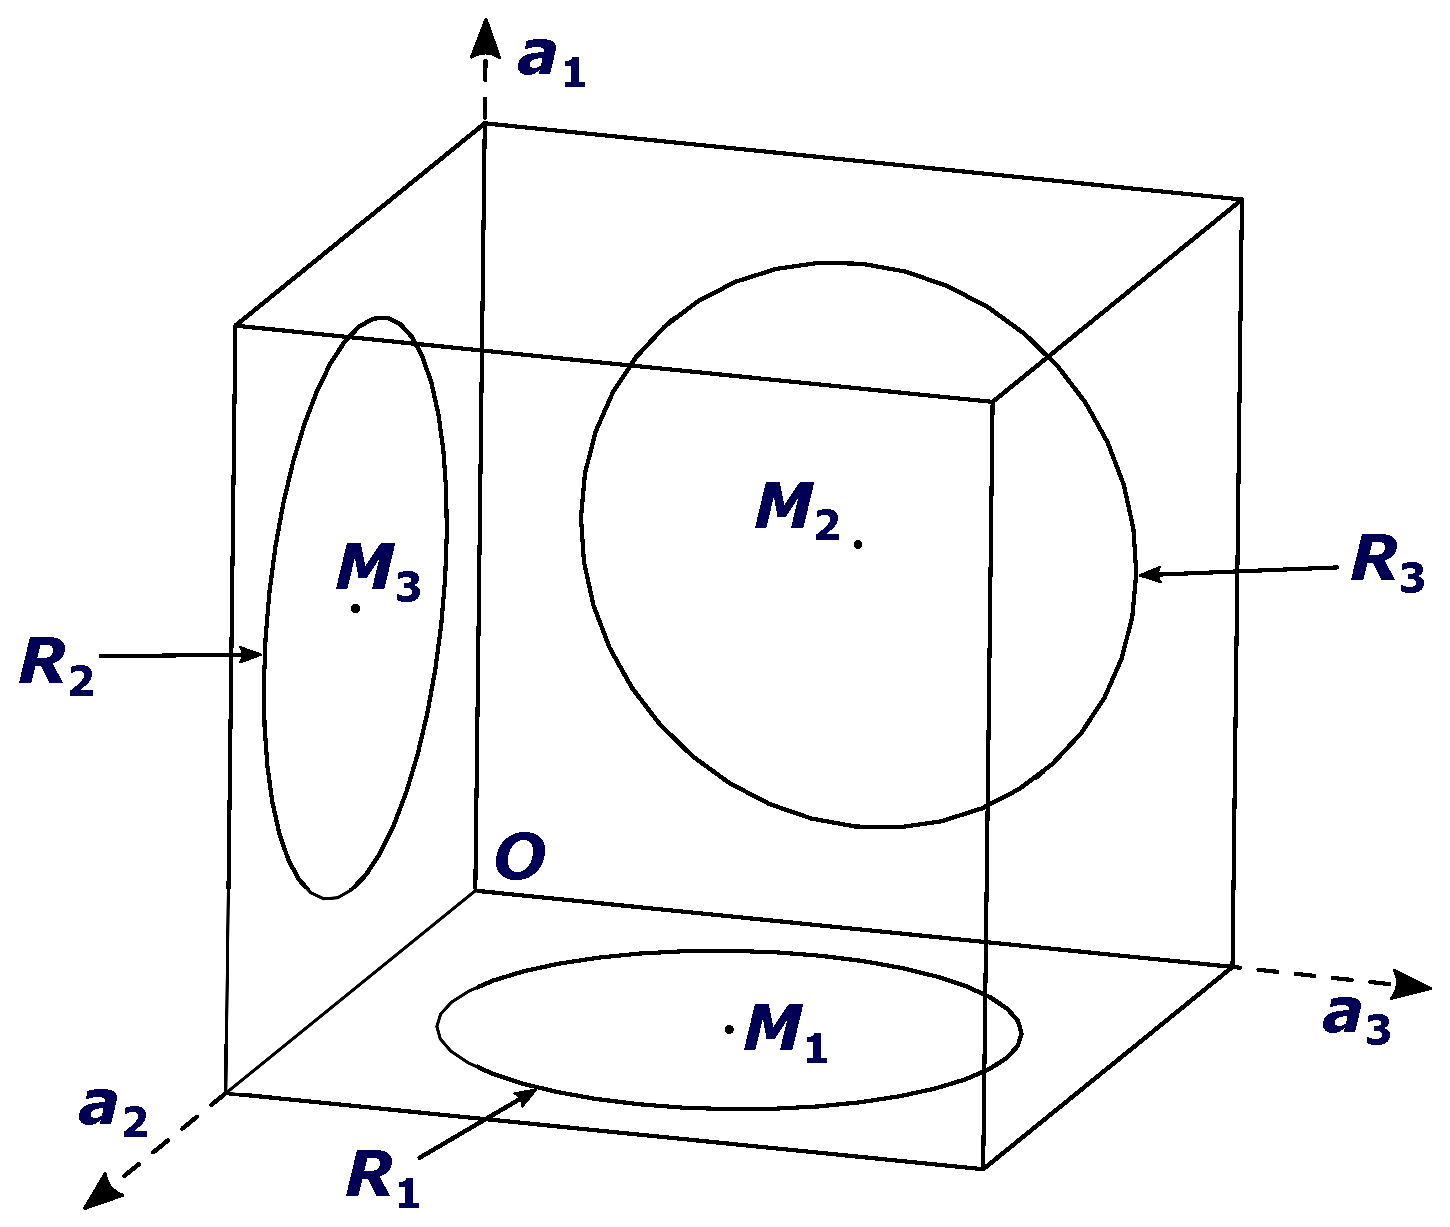
\includegraphics[width=0.75\textwidth]{img/tm_corner_drawing.eps}
\caption{Mechanische Skizze des Würfels}
\end{figure}
Durch die Rotation des Würfels um den Winkel $\varphi\idx1$ in Richtung des Vektors $\bs{a}\idx1$ entsteht das Hilfsbezugssystem $B$, welches durch die Einheitsvektoren $\bs{b}\idx1$, $\bs{b}\idx2$ und $\bs{b}\idx3$ definiert wird. Für die Abbildungsmatrix gilt
\begin{equation}
\pMat{A}{B} = \begin{bmatrix}
1 & 0 & 0 \\ 0 & c_{\varphi\idx1} & s_{\varphi\idx1} \\ 0 & -s_{\varphi\idx1} & c_{\varphi\idx1}
\end{bmatrix} \,.
\end{equation}
Die Rotation um den Winkel $\varphi\idx2$ in Richtung des Vektors $\bs{b}\idx2$ führt zu dem zweiten Hilfsbezugssystem $C$ mit den drei Einheitsvektoren $\bs{c}\idx1$, $\bs{c}\idx2$ und $\bs{c}\idx3$ sowie zu der Projektionsmatrix
\begin{equation}
\pMat{B}{C} = \begin{bmatrix}
c_{\varphi\idx2} & 0 & -s_{\varphi\idx2} \\
0 & 1 & 0 \\
 s_{\varphi\idx2} & 0 & c_{\varphi\idx2}
\end{bmatrix} \,.
\end{equation}
Die letzte Rotation des Würfels in Richtung des Vektors $\bs{c}\idx3$ um den Winkel $\varphi\idx3$ führt zu dem, durch die drei Vektoren $\bs{k}\idx1$, $\bs{k}\idx2$ und $\bs{k}\idx3$ definierten, Bezugssystem $K$. Für die Abbildungsmatrix gilt 
\begin{equation}
\pMat{C}{K} = \begin{bmatrix}
c_{\varphi\idx3} & s_{\varphi\idx3} & 0 \\ -s_{\varphi\idx3} & c_{\varphi\idx3} & 0 \\ 0 & 0 & 1
\end{bmatrix} \,.
\end{equation}
Hier sei angemerkt, dass es sich bei den Bezugssystemen $B$ und $C$ um theoretische Konstrukte handelt, für die kein physisches Gegenstück existiert. Sie werden lediglich als Hilfsmittel zur Beschreibung des Systems verwendet \cite[S. 24 ff.]{KaneBook}.

Durch die Rotation der Schwungmassen besitzt das System drei weitere Freiheitsgrade, welche von den Winkeln $\psi\idx1$, $\psi\idx2$ und $\psi\idx3$ beschrieben werden. Somit entstehen drei entsprechende Bezugssysteme, deren Vektorbasen jeweils an den Schwungmassen fixiert sind. Allerdings spielen diese keine weitere Rolle, da es sich bei den Winkeln $\psi_i$ um zyklische Koordinaten handelt. Das heißt, dass der Impuls des Systems nicht von der Ausrichtung der Schwungmassen beeinflusst wird. Lediglich die Winkelgeschwindigkeiten $\dot{\psi}_i$ wirken auf Grund der Reibung auf das System.

Die Position und Ausrichtung des Systems wird von den sechs Winkeln $\varphi_i$ und $\psi_i$ vollständig beschrieben, weshalb diese als generalisierte Koordinaten 
\begin{equation}
q_i \equiv \varphi_i \hspace{35pt} q_j \equiv \psi_i \hspace{35pt} (i=1,2,3, j=4,5,6) 
\end{equation}
definiert werden. Mit Hilfe der Bezugssysteme und generalisierten Koordinaten können nun die Winkelgeschwindigkeit des Würfels $\vel{A}{\omega}{K}$ und der Schwungmassen $\vel{A}{\omega}{R_i}$ bestimmt werden, welche sich aus der Addition der relativen Rotationsgeschwindigkeiten der Bezugssysteme zueinander ergeben \cite[S. 24]{KaneBook}.
\begin{equation}
\begin{split}
\vel{A}{\omega}{K} &= \vel{A}{\omega}{B}+\vel{B}{\omega}{C}+\vel{C}{\omega}{K} = \vecBS{A}{\dot{\varphi}\idx1}{0}{0} + \vecBS{B}{0}{\dot{\varphi}\idx2}{0} + \vecBS{C}{0}{0}{\dot{\varphi}\idx3} \\
&= \vecBS{K}
{\dot{\varphi}\idx2\cdot s_{\varphi\idx3} + \dot{\varphi}\idx1 \cdot c_{\varphi\idx2}\cdot c_{\varphi\idx3}}
{\dot{\varphi}\idx2\cdot c_{\varphi\idx3} - \dot{\varphi}\idx1 \cdot c_{\varphi\idx2}\cdot s_{\varphi\idx3}}
{\dot{\varphi}\idx3 + \dot{\varphi}\idx1\cdot s_{\varphi\idx2}}
\end{split}
\end{equation}
Die Winkelgeschwindigkeiten der Schwungmassen $\vel{K}{\omega}{R_i}$ relativ zu dem Würfel entsprechen der ersten Ableitung der Winkel $\psi_i$. Mit Hilfe des Additionstheorems für Winkelgeschwindigkeiten kann daraus auch die absolute Winkelgeschwindigkeit der Schwungmassen 
\begin{equation}
\vel{K}{\omega}{R_1} = \vecBS{K}{\dot{\psi}\idx1}{0}{0} \hspace{35pt}
\vel{K}{\omega}{R_2} = \vecBS{K}{0}{\dot{\psi}\idx2}{0} \hspace{35pt}
\vel{K}{\omega}{R_3} = \vecBS{K}{0}{0}{\dot{\psi}\idx3} 
\end{equation}
\begin{equation}
\vel{A}{\omega}{R_i} = \vel{A}{\omega}{K} + \vel{K}{\omega}{R_i} \hspace{35pt} (i=1,2,3)
\end{equation}
berechnet werden. Im nächsten Schritt werden die absoluten Geschwindigkeiten der Teilsysteme in Komponenten zerlegt, welche sich aus den generalisierten Geschwindigkeiten $u_i$ und partiellen Geschwindigkeiten $\vel{A}{\omega}{j}_i$ zusammensetzen. Hierfür müssen zunächst die generalisierten Geschwindigkeiten $u_i$ definiert werden. An dieser Stelle sei erwähnt, dass die Definition der generalisierten Geschwindigkeiten die Form der resultierenden Bewegungsgleichungen stark beeinflusst. Das letztendliche Ziel bei der Wahl der generalisierten Geschwindigkeiten ist es möglichst einfache Bewegungsgleichungen zu erhalten. Dies wird erreicht, indem die generalisierten Geschwindigkeiten so gewählt werden, dass sich die Geschwindigkeiten der Körper im Intertialsystem auf möglichst einfache Terme reduzieren lassen \cite{KanePaper}. Nach diesem Ansatz werden die  generalisierten Geschwindigkeiten 
\begin{equation}
\begin{split}
u\idx1 &= \dot{\varphi}\idx2\cdot s_{\varphi\idx3} + \dot{\varphi}\idx1\cdot c_{\varphi\idx2}\cdot c_{\varphi\idx3} \\
u\idx2 &= \dot{\varphi}\idx2\cdot c_{\varphi\idx3} - \dot{\varphi}\idx1\cdot c_{\varphi\idx2}\cdot s_{\varphi\idx3} \\
u\idx3 &= \dot{\varphi}\idx3 + \dot{\varphi}\idx1\cdot s_{\varphi\idx2} \\
u_4 &= \dot{\varphi}\idx2\cdot s_{\varphi\idx3} + \dot{\varphi}\idx1\cdot c_{\varphi\idx2}\cdot c_{\varphi\idx3} + \dot{\psi}\idx1 \\
u_5 &= \dot{\varphi}\idx2\cdot c_{\varphi\idx3} - \dot{\varphi}\idx1\cdot c_{\varphi\idx2}\cdot s_{\varphi\idx3} + \dot{\psi}\idx2 \\
u_6 &= \dot{\varphi}\idx3 + \dot{\varphi}\idx1\cdot s_{\varphi\idx2} + \dot{\psi}\idx3
\end{split}
\end{equation}
gewählt. Mit diesen Definitionen können die Winkelgeschwindigkeiten der Körper in A in die Form 
\begin{equation}
\vel{A}{\omega}{K} = \vecBS{K}{u\idx1}{u\idx2}{u\idx3}, \vel{A}{\omega}{R1} = \vecBS{K}{u\idx4}{u\idx2}{u\idx3}, \vel{A}{\omega}{R2} = \vecBS{K}{u\idx1}{u\idx5}{u\idx3}, \vel{A}{\omega}{R3} = \vecBS{K}{u\idx1}{u\idx2}{u\idx6}
\end{equation}
gebracht werden. Die Einführung der generalisierten Geschwindigkeiten führt einerseits zu einem einfachen  Ausdruck der absoluten Winkelgeschwindigkeiten aus Perspektive des körperfesten Bezugssystem $K$, andererseits können dadurch auch die partiellen Geschwindigkeiten $\vel{A}{\omega}{j}_i$ in einfachen Termen ausgedrückt werden. Für diese gilt 
\begin{align}
\vel{A}{\omega}{K} &= u\idx1 \cdot \bs{k}\idx1 + u\idx2 \cdot \bs{k}\idx2 + u\idx3 \cdot \bs{k}\idx3 &\rArrow &\vel{A}{\omega}{K}\idx1 = \bs{k}\idx1, \vel{A}{\omega}{K}\idx2 = \bs{k}\idx2, \vel{A}{\omega}{K}\idx3 = \bs{k}\idx3 \\
& & &\vel{A}{\omega}{K}\idx4 = 0, \vel{A}{\omega}{K}\idx5 = 0, \vel{A}{\omega}{K}\idx6 = 0 \nonumber
\\
\vel{A}{\omega}{R\idx1} &= u\idx4 \cdot \bs{k}\idx1 + u\idx2 \cdot \bs{k}\idx2 + u\idx3 \cdot \bs{k}\idx3 &\rArrow 
&\vel{A}{\omega}{K}\idx1 = 0, \vel{A}{\omega}{K}\idx2 = \bs{k}\idx2, \vel{A}{\omega}{K}\idx3 = \bs{k}\idx3 \\
& & &\vel{A}{\omega}{K}\idx4 = \bs{k}\idx1, \vel{A}{\omega}{K}\idx5 = 0, \vel{A}{\omega}{K}\idx6 = 0 \nonumber
\\
\vel{A}{\omega}{R\idx2} &= u\idx1 \cdot \bs{k}\idx1 + u\idx5 \cdot \bs{k}\idx2 + u\idx3 \cdot \bs{k}\idx3&\rArrow 
&\vel{A}{\omega}{K}\idx1 = \bs{k}\idx1, \vel{A}{\omega}{K}\idx2 = 0, \vel{A}{\omega}{K}\idx3 = \bs{k}\idx3 \\
& & &\vel{A}{\omega}{K}\idx4 = 0, \vel{A}{\omega}{K}\idx5 = \bs{k}\idx2, \vel{A}{\omega}{K}\idx6 = 0 \nonumber
\\
\vel{A}{\omega}{R\idx3} &= u\idx1 \cdot \bs{k}\idx1 + u\idx2 \cdot \bs{k}\idx2 + u\idx6 \cdot \bs{k}\idx3&\rArrow 
&\vel{A}{\omega}{K}\idx1 = \bs{k}\idx1, \vel{A}{\omega}{K}\idx2 = \bs{k}\idx2, \vel{A}{\omega}{K}\idx3 = 0 \\
& & &\vel{A}{\omega}{K}\idx4 = 0, \vel{A}{\omega}{K}\idx5 = 0, \vel{A}{\omega}{K}\idx6 = \bs{k}\idx3 \nonumber \,.
\end{align}
Die Bedeutung der generalisierten und partiellen Geschwindigkeiten kann als eine Unterteilung der Bewegung in Betrag und Richtung interpretiert werden. Die generalisierten Geschwindigkeiten geben als skalare Größen den Betrag der Geschwindigkeit wieder, wobei die entsprechenden partiellen Geschwindigkeiten die Bewegungsrichtung darstellen.
